\documentclass[]{article}

\usepackage{color}
\usepackage{amsmath}
\usepackage{amssymb}
\usepackage{graphicx}
\graphicspath{{./figure/}}
\definecolor{gray}{RGB}{216,216,216}

% Title Page
\title{}
\author{Miao Li}


\begin{document}
\maketitle

\begin{abstract}
\end{abstract}

\section{Introduction}
In this report, we address the problem of variable stiffness control for robust grasping. As shown in our previous work (\textcolor{red}{IROS2014}), variable stiffness control can effectively stabilize the grasp under disturbance. However, the stability of such controller has never been addressed before. In this work, we are trying to address this problem using a two-fingered test examples,see Fig.~\ref{fig::system}.
To this end, first, a detailed formulation for the dynamics of the hand-object is derived, which takes rolling constraints and the soft fingertip into account. Then, a variable stiffness controller is presented to grasp the object stable and the upper bound for the change rate of the stiffness is derived from the proof of stability.
\textcolor{red}{(We follow the same notation as in Arimoto's book, add ref.)}
\begin{figure}[h!]
\centering
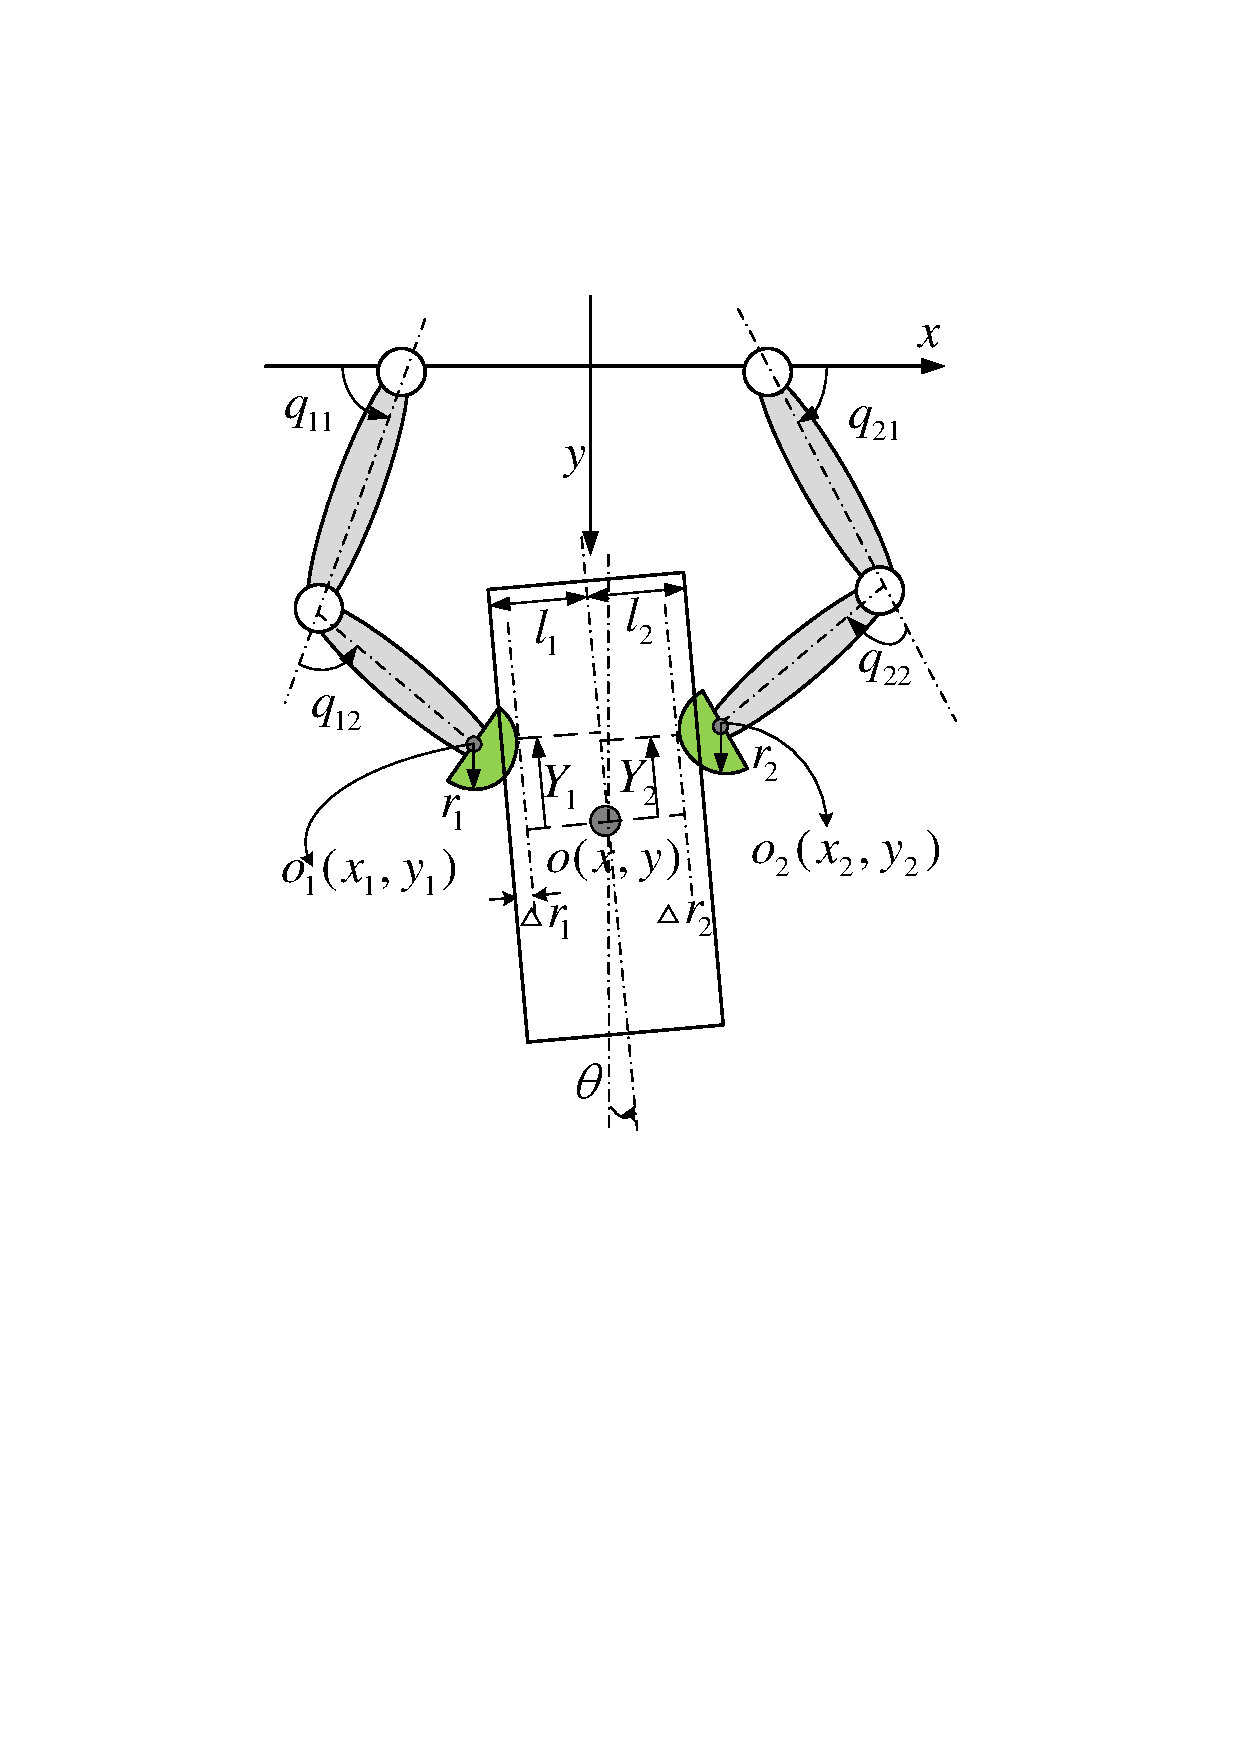
\includegraphics[height=7cm]{hand_object_system.pdf}
\caption{The hand-object system in 2D. Each finger has 2 DOFs with soft fingertips.}
\label{fig::system}
\end{figure}

\section{Dynamics}
In this part, we first consider the contact model of the fingertips and the constraints involved in the hand-object system. Then the overall dynamics of the system is formulated. 
\subsection{Contact model of soft fingertip}
\begin{equation}
f=c_1(\Delta r)^2+ c_2\frac{d}{dt}\Delta r
\end{equation}
where $c_1$ and $c_2$ are positive constant parameters which depends on the material of the fingertip.
\subsection{Contact constraints}
\begin{figure}[h!]
\centering
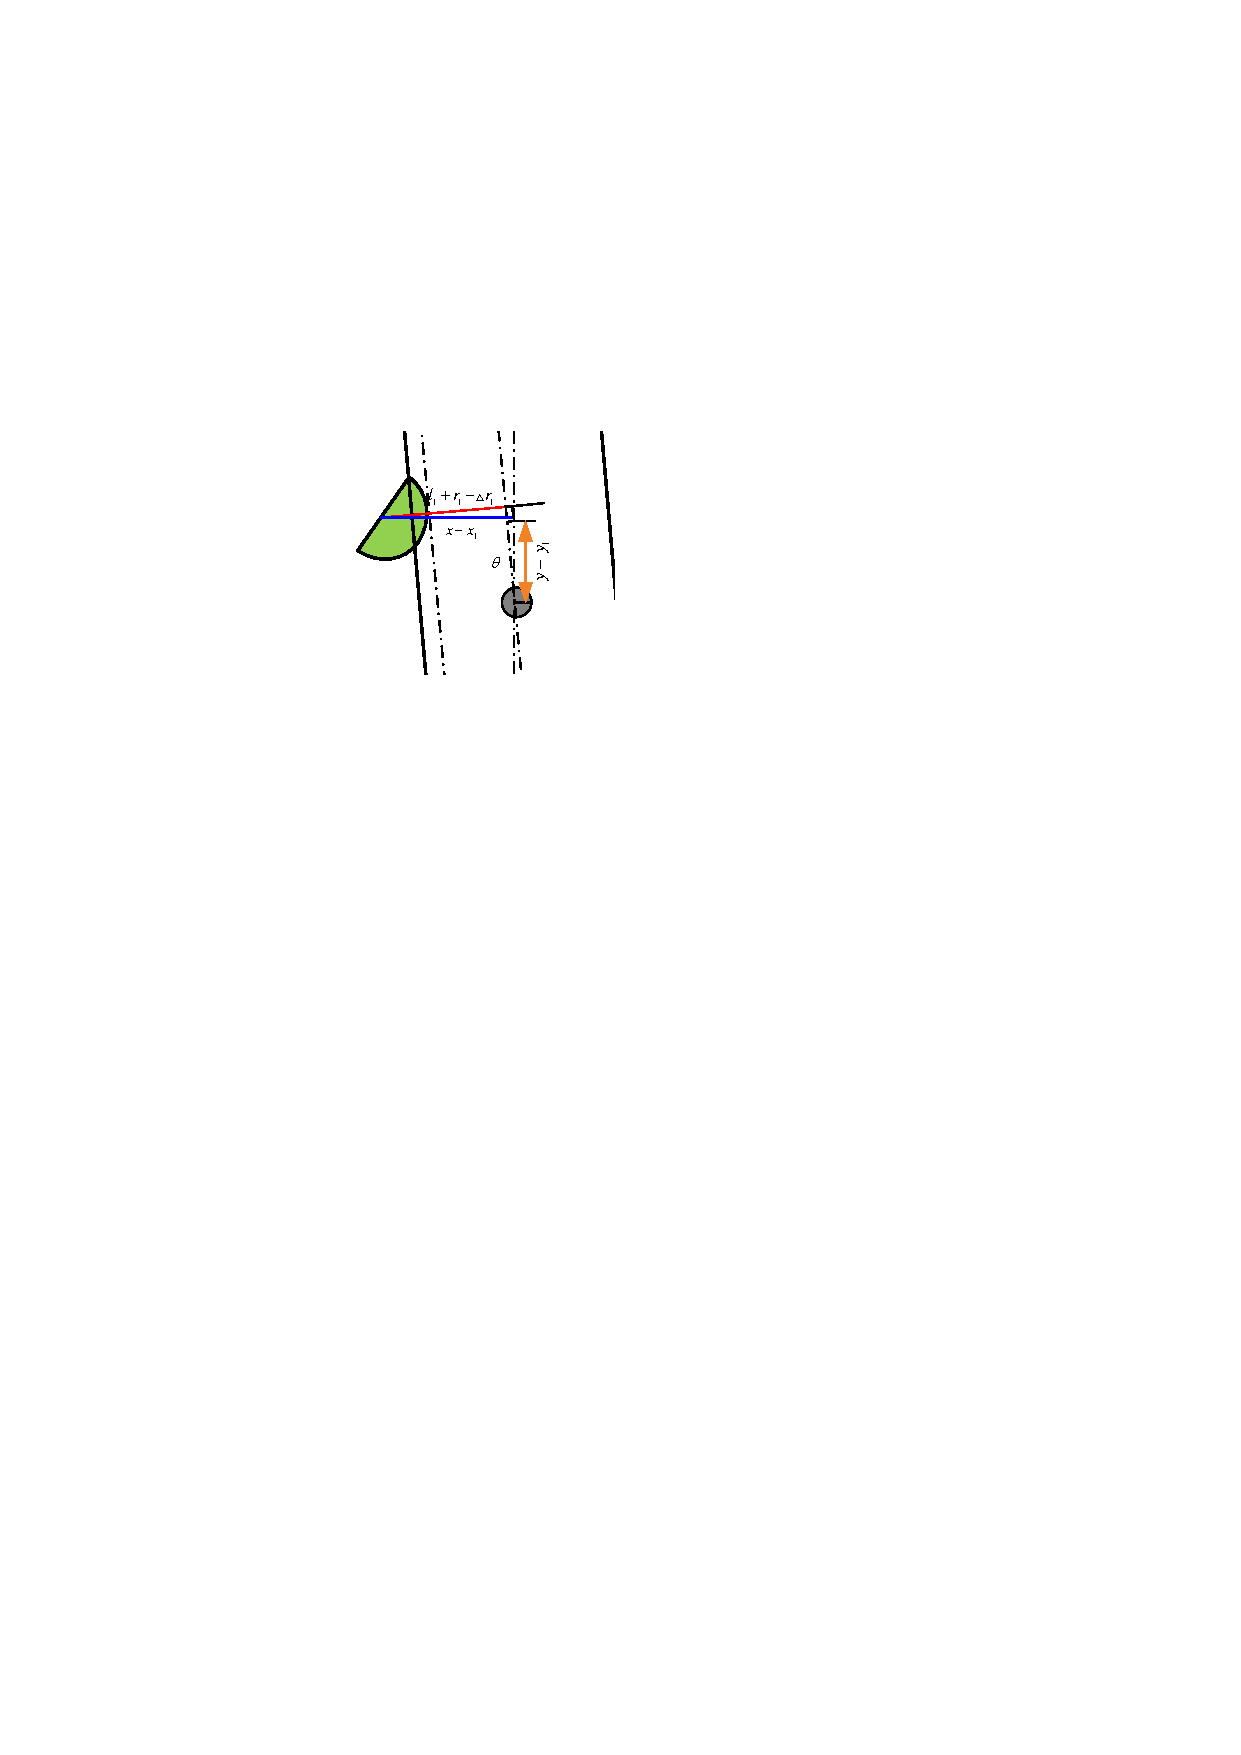
\includegraphics[height=5cm]{hand_object_cons1.pdf}
\caption{The constraint that the fingertip should keep contact with the object surface.}
\label{fig::cons1}
\end{figure}
The fingertip should keep contact with the object surface, as shown in Fig.~\ref{fig::cons1}, which can be expressed as follows:
\begin{equation}
l_1+r_1-\Delta r_1=(x-x_1)\cos\theta-(y-y_1)\sin\theta
\label{eqn::cons_contact1}
\end{equation}
\begin{equation}
l_2+r_2-\Delta r_2=-(x-x_2)\cos\theta+(y-y_2)\sin\theta
\label{eqn::cons_contact2}
\end{equation}
\subsection{Rolling constraints}
The rolling constraints on each fingertip can be represented as:
\begin{equation}
(r_i-\Delta r_i)\frac{d}{dt}\phi_i=-\frac{d}{dt}Y_i,\quad i=1,2
\label{eqn::cons_rolling}
\end{equation}
where $Y_i$ and $\phi_i$ are given by:
\begin{equation}
Y_i=(x_i-x)\sin\theta+(y_i-y)\cos\theta
\end{equation}
\begin{equation}
q_{11}+q_{12}+\phi_1=\pi+\theta
\end{equation}
\begin{equation}
q_{21}+q_{22}+\phi_2=\pi-\theta
\end{equation}
\subsection{Overall Dynamics}
The total kinetic energy for the overall system can be described as follows:
\begin{equation}
K=\sum\limits_{i=1,2}\frac{1}{2}\mathbf{\dot{q}}_i^TH_i\mathbf{\dot{q}}_i+\frac{1}{2}
M(\dot{x}^2+\dot{y}^2)+\frac{1}{2}I\dot{\theta}^2
\end{equation}
where $\mathbf{q}_i=[q_{i1},q_{i2}]^T$.

The total potential energy can be given as:
\begin{equation}
P=\sum\limits_{i=1,2}\int_{0}^{\Delta r_i}c_1\eta^2d\eta
\end{equation}
Then from the Hamilton's principle, we have:
\begin{equation}
\int_{t_0}^{t_1}\left[\delta(K-P)-\sum\limits_{i=1,2}c_2\Delta \dot{r}_i
\frac{\partial\Delta r_i}{\partial X^T}\delta X + \sum\limits_{i=1,2}\lambda_i[(r_i-\Delta r_i)\frac{\partial\phi_i}{\partial X^T} + \frac{\partial Y_i}{\partial X^T}]\delta X +\sum\limits_{i=1,2}\mathbf{u_i}^T\delta \mathbf{q}_i\right]dt=0
\end{equation}
where $X=[\mathbf{q}_1^T,\mathbf{q}_2^T,x,y,\theta]^T$.

Then we have the overall dynamics for the object-hand system as follows:
\begin{equation}
H_i(\mathbf{q_i})\ddot{\mathbf{q}}_i+(\frac{1}{2}\dot{H}_i+S_i)\mathbf{\dot{q}}_i+f_i
\frac{\partial \Delta r_i}{\partial \mathbf{q}_i^T}-\lambda_i[(r_i-\Delta r_i)\frac{\partial\phi_i}{\partial \mathbf{q}_i^T} + \frac{\partial Y_i}{\partial \mathbf{q}_i^T}]=\mathbf{u}_i
\end{equation}
\begin{equation}
M\ddot{x}+\sum\limits_{i=1,2}[f_i\frac{\partial \Delta r_i}{\partial x}-\lambda_i
\frac{\partial Y_i}{\partial x}]=0
\end{equation}
\begin{equation}
M\ddot{y}+\sum\limits_{i=1,2}[f_i\frac{\partial \Delta r_i}{\partial y}-\lambda_i
\frac{\partial Y_i}{\partial y}]=0
\end{equation}
\begin{equation}
I\ddot{\theta}+\sum\limits_{i=1,2}[f_i\frac{\partial \Delta r_i}{\partial \theta}-\lambda_i((r_i-\Delta r_i)\frac{\partial\phi_i}{\partial \theta}+
\frac{\partial Y_i}{\partial \theta})]=0
\end{equation}

With the identities in appendix \ref{sec::app1}, the overall dynamics can be simplified as:
\begin{equation}
H_i(\mathbf{q_i})\ddot{\mathbf{q}}_i+(\frac{1}{2}\dot{H}_i+S_i)\mathbf{\dot{q}}_i-(-1)^if_iJ_i^T\begin{bmatrix}
\cos\theta\\
-\sin\theta
\end{bmatrix}-\lambda_i[(r_i-\Delta r_i)\begin{bmatrix}
-1\\-1
\end{bmatrix} + J_i^T\begin{bmatrix}
\sin\theta\\\cos\theta
\end{bmatrix}=\mathbf{u}_i
\end{equation}

\begin{equation}
M\ddot{x}-(f_1-f_2)\cos\theta+(\lambda_1+\lambda_2)\sin\theta=0
\end{equation}
\begin{equation}
M\ddot{y}+(f_1-f_2)\sin\theta+(\lambda_1+\lambda_2)\cos\theta = 0
\end{equation}
\begin{equation}
I\ddot{\theta}-f_1Y_1+f_2Y_2+l_1\lambda_1-l_2\lambda_2=0
\end{equation}
\section{Variable stiffness control}
Motivated by the analysis of the overall system dynamics, the following control law is adopted for each finger to achieve stable grasp:
\begin{equation}
u_i=-D_i\mathbf{\dot{q}}_i+kJ_i^T(\mathbf{x}_i-\mathbf{x}_d)
\label{eqn::control}
\end{equation}
\begin{align}
&\mathbf{x}_i=\begin{bmatrix}
x_i\\
y_i
\end{bmatrix}
&\mathbf{x}_d=\frac{1}{2}\begin{bmatrix}
x_1+x_2\\
y_1+y_2
\end{bmatrix}
\end{align}
where $D_i$ is a diagonal positive definite matrix representing the damping gain. $k\in R^+$ represents the \emph{variable} stiffness for each fingertip($k$ is the same value for the two-finger grasp to ensure force balance).

\section{Stability Proof--1}
Taking the sum of inner product of (15) with $\mathbf{\dot{q_i}},i=1,2$, (16) with $\dot{x}$, (17) with $\dot{y}$, (18) with $\dot{\theta}$, we have:
\begin{equation}
\frac{d}{dt}E=-\sum\limits_{i=1,2}\{\mathbf{\dot{q}}_i^TD_i\mathbf{\dot{q}}_i+c_2\Delta \dot{r}_i^2\}+\frac{\dot{k}}{4}{(\mathbf{x}_1-\mathbf{x}_2)^T(\mathbf{x}_1-\mathbf{x}_2)}
\label{eqn::dE}
\end{equation}
\begin{equation}
E=K+V+P
\end{equation}
\begin{equation}
K=\sum\limits_{i=1,2}\frac{1}{2}\mathbf{\dot{q}}_i^TH_i\mathbf{\dot{q}}_i+\frac{1}{2}
M(\dot{x}^2+\dot{y}^2)+\frac{1}{2}I\dot{\theta}^2
\end{equation}
\begin{equation}
P=\sum\limits_{i=1,2}\int_{0}^{\Delta r_i}c_1\eta^2d\eta
\end{equation}
\begin{equation}
V=\frac{k}{4}(\mathbf{x}_1-\mathbf{x}_2)^T(\mathbf{x}_1-\mathbf{x}_2)
\end{equation}
\textcolor{red}{As proved in Arimoto's book, the closed-loop dynamics is asymptotically stable if:}
\begin{equation}
\frac{d}{dt}E<0
\end{equation}•
which leads to
\begin{equation}
\dot{k}<\frac{\sum\limits_{i=1,2}\{\mathbf{\dot{q}}_i^TD_i\mathbf{\dot{q}}_i+c_2\Delta \dot{r}_i^2\}}{(\mathbf{x}_1-\mathbf{x}_2)^T(\mathbf{x}_1-\mathbf{x}_2)}
\end{equation}
From this, we can conclude the following comments \textcolor{red}{Is this conclusion correct? Any example?}:
\begin{itemize}
\item If the object is softer, $c_2$ is bigger, we can change the stiffness faster.
\item If the object is smaller, $(\mathbf{x}_1-\mathbf{x}_2)^T(\mathbf{x}_1-\mathbf{x}_2)$, we can change the stiffness faster
\end{itemize}
\textcolor{red}{As noticed that the change rate of the stiffness is still depending on the state variable and we still don't know how wo realize the desired stiffness. Note: in our previous work of grasp adaptation, we simply change the $k$ to $k_d$, which may lead to unstable behavior if $k_d-k$ is too big. This leads us to the following section.}

\section{Stability Proof}
The stability proof in previous section set an upper bound for the change rate of stiffness. However, it does not take the control policy for the stiffness into account. In our IROS paper, the desired stiffness is a function of the tactile sensing $S$ and the rest length $L$, which is encoded using a probabilistic model GMM as follows,

\begin{equation}
k=g(S,L)=\sum_{i=1}^{m}h_i[\mu_{k,i}+\Sigma_{ky,i}\Sigma^{-1}_{y,i}(y-\mu_{y,i})]
\label{eqn::GMM_K}
\end{equation}    
Denote $y=[L^T,S^T]^T$, \textcolor{red}{Explain all the notations here later}. \\
To prove eqn.~(\ref{eqn::dE}), we need to compute the change rate of stiffness, i.e. $\dot k$,
\begin{align}
\dot k &= \frac{\partial k}{\partial y}(\frac{\partial y}{\partial L}\frac{\partial L}{\partial t}+\frac{\partial y}{\partial s}\frac{\partial s}{\partial t}) \\
&=\frac{\partial k}{\partial y}\begin{bmatrix}
\mathbf{x}_1^TJ_1\mathbf{\dot q}_1+\mathbf{x}_2^TJ_2\mathbf{\dot q}_2\\
\mathbf{x}_1^TJ_1\mathbf{\dot q}_1+\mathbf{x}_2^TJ_2\mathbf{\dot q}_2\\
\frac{\partial s}{\partial t}2\|\mathbf{x}_1-\mathbf{x}_2\|
\end{bmatrix}\frac{1}{2\|\mathbf{x}_1-\mathbf{x}_2\|}
\end{align}

From the definition of eqn.~(\ref{eqn::GMM_K}), we have:
\begin{equation}
\frac{\partial k}{\partial y} = \sum_{i=1}^{m}\{\frac{\partial h_i}{\partial y}[\mu_{k,i}+\Sigma_{ky,i}\Sigma^{-1}_{y,i}(y-\mu_{y,i})]+h_i(\Sigma_{ky,i}\Sigma^{-1}_{y,i})\}
\end{equation}

\textcolor{red}{Key Assumption:} During the change of stiffness, we assume the weight of each gaussian components does not change with respect to $y$, namely $\frac{\partial h_i}{\partial y}=0$.

We shall view $h_i$ as the responsibility of the $i-$ gaussian component, but only use the rest length to compute it. Due to the physical constraints of the grasp, during the change of stiffness, the rest length doesn't change (ignoring the effect of fingertip's deformation) and thus it is more reliable to just the rest length for computing the weighting coefficients $h_i$. Therefore we have $\frac{\partial h_i}{\partial y}=0$.
 
With this assumption, we have:
\begin{align}
\frac{\partial k}{\partial y} &= \sum_{i=1}^{m}h_i(\Sigma_{ky,i}\Sigma^{-1}_{y,i})\\
 & :=[A_{11},A_{12},A_{13}]
\end{align}
Note that $A_{11},A_{12},A_{13}$ are constant values.
To prove $\frac{d}{dt}E<0$, we only need to proove:
\begin{align}
&[A_{11},A_{12},A_{13}]*\begin{bmatrix}
\mathbf{x}_1^TJ_1\mathbf{\dot q}_1+\mathbf{x}_2^TJ_2\mathbf{\dot q}_2\\
\mathbf{x}_1^TJ_1\mathbf{\dot q}_1+\mathbf{x}_2^TJ_2\mathbf{\dot q}_2\\
\frac{\partial s}{\partial t}*2\|\mathbf{x}_1-\mathbf{x}_2\|
\end{bmatrix}\frac{1}{2\|\mathbf{x}_1-\mathbf{x}_2\|}*\frac{\|\mathbf{x}_1-\mathbf{x}_2\|^2}{4}-\sum\limits_{i=1,2}\{\mathbf{\dot{q}}_i^TD_i\mathbf{\dot{q}}_i+c_2\Delta \dot{r}_i^2\}<0\\
&\Leftarrow (A_{11}+A_{12})\mathbf{x_1}^TJ_1\mathbf{\dot q}_1+(A_{11}+A_{12})\mathbf{x_2}^TJ_2\mathbf{\dot q}_2+A_{13}\frac{\partial s}{\partial t}2\|\mathbf{x}_1-\mathbf{x}_2\|< \nonumber\\
&\mathbf{\dot q}_1^T\frac{2D_1}{\|\mathbf{x}_1-\mathbf{x}_2\|}\mathbf{\dot q}_1+\mathbf{\dot q}_2^T\frac{2D_2}{\|\mathbf{x}_1-\mathbf{x}_2\|}\mathbf{\dot q}_2 \quad +2\sum\limits_{i=1,2}\{c_2\Delta \dot{r}_i^2\}/\|\mathbf{x}_1-\mathbf{x}_2\|\\
&\Leftarrow A_{13}\frac{\partial s}{\partial t}<\mathbf{\dot q}_1^T\frac{D_1}{\|\mathbf{x}_1-\mathbf{x}_2\|^2}\mathbf{\dot q}_1-\frac{A_{11}+A_{12}}{2\|\mathbf{x}_1-\mathbf{x}_2\|}\mathbf{x_1}^TJ_1\mathbf{\dot q}_1+ \nonumber\\
&~~~~~~~~~~~~~~~~\mathbf{\dot q}_2^T\frac{D_1}{\|\mathbf{x}_1-\mathbf{x}_2\|^2}\mathbf{\dot q}_2-\frac{A_{11}+A_{12}}{2\|\mathbf{x}_1-\mathbf{x}_2\|}\mathbf{x_2}^TJ_2\mathbf{\dot q}_2+\sum\limits_{i=1,2}\{c_2\Delta \dot{r}_i^2\}/\|\mathbf{x}_1-\mathbf{x}_2\|^2\\
&\Leftarrow A_{13}\frac{\partial s}{\partial t}+ (\frac{A_{11}+A_{12}}{4})^2[\mathbf{x}_1^TJ_1D_1^{-1}J_1^T\mathbf{x}_1+\mathbf{x}_2^TJ_2D_2^{-1}J_2^T\mathbf{x}_2]< \nonumber \\
&~~~~~~~~~~\underbrace{\| \frac{D_1^{-1/2}}{\|\mathbf{x}_1-\mathbf{x}_2\|}\mathbf{\dot q}_1-\mathbf{b}_1\|^2+\| \frac{D_2^{-1/2}}{\|\mathbf{x}_1-\mathbf{x}_2\|}\mathbf{\dot q}_2-\mathbf{b}_2\|^2+\sum\limits_{i=1,2}\{c_2\Delta \dot{r}_i^2\}/\|\mathbf{x}_1-\mathbf{x}_2\|^2}_{\text{denote this part as $\gamma$ and $\gamma>0$}}\\
&\Leftarrow A_{13}\frac{\partial s}{\partial t}+ (\frac{A_{11}+A_{12}}{4})^2[\mathbf{x}_1^TJ_1D_1^{-1}J_1^T\mathbf{x}_1+\mathbf{x}_2^TJ_2D_2^{-1}J_2^T\mathbf{x}_2]< \gamma \label{eqn::proof}
\end{align}
Note that the first term in the left side of eqn.~(\ref{eqn::proof})), i.e., $A_{13}\frac{\partial s}{\partial t}$ represents the change of stiffness due to the change of tactile sensing, if it is negative, eqn.~(\ref{eqn::proof})) will keep holding and we don't need to change the damping to stabilize the system. When $A_{13}\frac{\partial s}{\partial t}>0$, namely increasing the stiffness according to the tactile sensing, we need to set a proper damping term to stabilize the system.
From the bound of Jacobian(Christian ott's book), we have,
\begin{equation}
\lambda_{max}(J_iJ_i^T)<\sigma_{max}^2, i=1,2
\end{equation}
Also, from the physical constraint of the finger, $\|\mathbf{x}_i\|<L_f, i=1,2$. Assume we use the same damping at each joint, $D_1=D_2=diag\{d_i\}$, then we have:
\begin{equation}
\end{equation}

\section{Stability Proof--2}
As noticed in Eq. \ref{eqn::dE}, the dissipated energy $\sum\limits_{i=1,2}\{\mathbf{\dot{q}}_i^TD_i\mathbf{\dot{q}}_i+c_2\Delta \dot{r}_i^2\}$ set an upper bound for the energy that we can inject into the system. In order to stably vary the stiffness, we keep track of the energy dissipated by the system using a virtual tank(\textcolor{red}{add ref.}). The control signal is designed as follows:
\begin{equation}
u_i=-D_i\mathbf{\dot{q}}_i+J_i^T(\omega z)
\label{eqn::new_control}
\end{equation} 
The new term $z\in \mathbb{R}$ is the state variable associated with the energy in the tank and,
\begin{equation}
T(z)=\frac{1}{2}z^2
\end{equation}
\begin{equation}
\dot{z}=\frac{\sigma}{z}\sum\limits_{i=1,2}\{\mathbf{\dot{q}}_i^TD_i\mathbf{\dot{q}}_i+c_2\Delta \dot{r}_i^2\}-\sum\limits_{i=1,2}\omega^T J_i\mathbf{\dot{q_i}}
\end{equation}
$\omega(t)\in \mathbb{R}^3$ is the control variable through which it is possible to exchange the energy between the impedance components and the tank. $\sigma$ is a design parameter that opens/closes the tank for energy exchange:
\begin{displaymath}
\sigma = \left\{\begin{array}{ll}
1& T(z)<T_{lim}\\
0& otherwise
\end{array}\right.
\end{displaymath}
Now with the new controller and tank energy, we can derive:
\begin{equation}
E=K+V+T
\end{equation}
\begin{equation}
\frac{d}{dt}E=-\sum\limits_{i=1,2}\{\mathbf{\dot{q}}_i^TD_i\mathbf{\dot{q}}_i+c_2\Delta \dot{r}_i^2\}+\sigma\sum\limits_{i=1,2}\{\mathbf{\dot{q}}_i^TD_i\mathbf{\dot{q}}_i+c_2\Delta \dot{r}_i^2\}\leq0
\label{eqn::dE2}
\end{equation}
Recalling Eq. \ref{eqn::control}, to get the desired stiffness $k_d$, we can exploit the energy stored in the tank by setting:
\begin{displaymath}
\omega(t)=\left\{\begin{array}{ll}
K_d(\mathbf{x}_i-\mathbf{x}_d)/z & T(z)>T_{low}\\
0&otherwise
\end{array}\right.
\end{displaymath}
The stability proof is similar by following Arimoto's method from Eq. \ref{eqn::dE2}.
\section{simulation}
In this section, we will use an 1D example to example the idea of virtual tank for implementing the varying stiffness.

\section{appendix}
\appendix
\section{Identities}
\label{sec::app1}
From equation (2)(3)(5)(6)(7), we have the following identities:

\colorbox{gray}{
\begin{minipage}{9cm}
 \begin{align*}
 &\frac{\partial \Delta r_1}{\partial \mathbf{q}_1^T}=J_{1}^T\left[\cos\theta,-\sin\theta\right]^T 
 &\frac{\partial \Delta r_2}{\partial \mathbf{q}_2^T}=-J_{2}^T\left[\cos\theta,-\sin\theta\right]^T\nonumber\\
 &\frac{\partial \phi_1}{\partial \mathbf{q}_1^T}=[-1,-1]^T
 &\frac{\partial \phi_2}{\partial \mathbf{q}_2^T}=[-1,-1]^T\nonumber\\
 &\frac{\partial Y_1}{\partial\mathbf{q}_1^T}=J_1^T[\sin\theta,\cos\theta]^T
 &\frac{\partial Y_2}{\partial \mathbf{q}_2^T}=J_2^T[\sin\theta,\cos\theta]^T\nonumber\\
 &\frac{\partial \Delta r_1}{\partial x}=-\cos\theta
 &\frac{\partial \Delta r_2}{\partial x}=\cos\theta \nonumber\\
 &\frac{\partial Y_1}{\partial x}=-\sin\theta 
 &\frac{\partial Y_2}{\partial x}=-\sin\theta \nonumber\\
 &\frac{\partial \Delta r_1}{\partial y}=\sin\theta&\frac{\partial \Delta r_2}{\partial y}=-\sin\theta \nonumber\\
  &\frac{\partial Y_1}{\partial y}=-\cos\theta &\frac{\partial Y_2}{\partial y}=-\cos\theta \nonumber\\
  &\frac{\partial \Delta r_1}{\partial \theta}=-Y_1&\frac{\partial \Delta r_2}{\partial \theta}=Y_2\nonumber\\
  &\frac{\partial \phi_1}{\partial \theta}=1&\frac{\partial \phi_2}{\partial \theta}=-1\nonumber\\
  &\frac{\partial Y_1}{\partial \theta}=(x_1-x)\cos\theta-(y_1-y)\sin\theta&\\
  &\frac{\partial Y_2}{\partial \theta}=(x_2-x)\cos\theta-(y_2-y)\sin\theta&\nonumber
 \end{align*}
\end{minipage}}
\end{document}          
